\documentclass{article}
\usepackage[svgnames]{xcolor}
\usepackage[a0paper,landscape,margin=3cm]{geometry}
\usepackage[utf8]{inputenc}
\usepackage[sorting=nyt,backend=biber,style=authoryear,block=par]{biblatex}
\usepackage{anyfontsize}
\usepackage{tikz}
\usepackage{mathpazo}
\usepackage{multicol,caption}
\usepackage{tikz}
\usepackage{graphicx}
\usepackage[inkscapeformat=png]{svg}
\usepackage{blindtext}
\usepackage[inkscapeformat=png]{svg}
\usepackage{booktabs}
\usepackage{xurl}
\usetikzlibrary{matrix,fadings,arrows,trees,calc,positioning,decorations,automata,fit,backgrounds}
\pagecolor{red!5}

\columnsep=50pt
% \columnseprule=2pt
\graphicspath{ {images/} }



\renewcommand{\section}[1]{
    \begin{center}
        \begin{tikzpicture}
            \draw node[fill=white!10, text width=0.85\linewidth, text centered, inner sep=10pt, rounded corners=5pt, draw=red!80]
            {\textbf{#1}};
        \end{tikzpicture}
   
    \end{center}

}

\renewcommand{\bibfont}{}

% {\subsection*{References }}
\addbibresource{References.bib}


\renewcommand{\subsection}[1]{
    % \begin{center}
        % \begin{tikzpicture}
        %     \draw node[fill=white!10, text width=0.97\linewidth, text centered, inner sep=10pt, rounded corners=5pt, draw=red!30]
        %     {\textbf{#1}};
        % \end{tikzpicture}
        {\textbf{#1}}
    % \end{center}

}

\newenvironment{Figure}
  {\par\medskip\noindent\minipage{\linewidth}}
  {\endminipage\par\medskip}

\begin{document}

    \fontsize{50}{60}
    \selectfont
     \begin{tikzpicture}
            
        \node[inner sep=0pt] (logo) {\includesvg{SRH_Bildung.svg}}; 
        \draw node[text width=0.87\linewidth,text centered,rounded corners=5pt,inner sep=30pt,right=100pt of logo] (title){
            {Application of Natural Language Processing in an E-commerce industry}\\[0.5cm]
            \fontsize{50}{55}
            \selectfont
            {Predicting multilevel product category} \\[1cm]  
            \fontsize{40}{50}
            \selectfont
            Shoney Arickathil, Prof. Dr. Gerd Moeckel \\[0.5cm]
            \fontsize{50}{50}
            \selectfont
            Applied Computer Science, SRH Hochschule, Heidelberg
            };
    \begin{scope}[on background layer]
        \node [fill=Red!10, fit={(logo) (title)}] {};
    \end{scope}

\end{tikzpicture}
\vspace{1cm}
\begin{multicols*}{3}

   
    \fontsize{34}{36}
    \selectfont
 
    \section{Introduction}
    E-commerce sales are increasing exponentially ever since the world is connected online. Convenience for searching the desired product, comparing different products before making a purchase and easy access on tips of the finger has made online shopping trending especially among the youth. A vast variety of products are sold online.

    Product taxonomy (categorization) is the logical and hierarchical arrangement of the company's product. A well-defined product taxonomy enables customers to search the desired product in the least number of clicks on an E-commerce website. 
    An AI of unsupervised learning model to create product taxonomy based on product features is the need of the hour. In this paper, research on automating the process of defining the product taxonomy is conducted. 
    
 
    \section{Problem statement and objective}

    In a business to business(B2B) type of Ecommerce, the product taxonomy exchange between the companies such as suppliers and manufactures and online retailer may differ. Product taxonomy must be analyzed and fit into the existing vocabulary of the product taxonomy of online retailer. An example, if a supplier name a certain product category as "Engine oil" and the category already existing at online retailer is "Motor Oil". In such case importing the category from the supplier may result in poorly defined product taxonomy. The objective is to perform feature selection of product details using scikit learn \parencite{sklearn_api}, process text based classification on each hierarchy to predict the category levels of the product.

    \begin{multicols}{2}
        \section{Tools and Technologies}
            \includesvg{PyTorch_logo_black.svg} \\
            Pytorch  \parencite{Paszke.03122019} is a machine learning library which provides Pythonic programming style. The open-source Python ecosystem packages like NumPy, SciPy and Pandas fulfills most of the numerical analysis needs of research.  Python provides vast repositories of libraries to handle data preprocessing, statistical analysis and plotting. Pytorch performs execution of dynamic tensors computation with automatic differentiation for efficient gradient based optimization. 
                 
    \columnbreak
        \section{Research questions}
        \begin{enumerate}
            \item How Natural Language Processing (NLP) can be applied in ecommerce industry?
            \item Which neural network architecture is suitable for text based classification model?
            \item What are the steps involved for preprocessing text to extract features from the document?
            \item  How to get better results with better shaped network? Evaluate neural network performance based on confusion matrix.
        \end{enumerate}
     
    \end{multicols}

  \columnbreak
    \section{Methodology}
    \begin{enumerate}
        \item Inspiration: Unmanageable and not well-defined product taxonomy. 
        \item Empathize: Gained in depth understanding of the Ecommerce industries requirement.
        \item Ideate: Modifying Tutorial on character-level RNN \parencite{sean}  to work with vocabulary level RNN.
        \item Prototype: Creating a prototype of predicting category based on a single feature of product before including all the features.
        \item Test: Testing the prototype and gaining the feedback from the user. 
    \end{enumerate} 

    
    \vspace{0.5cm}
    \section{Network Architecture - Recurrent Neural Network}
    % \begin{Figure}
    %     \centering
    %     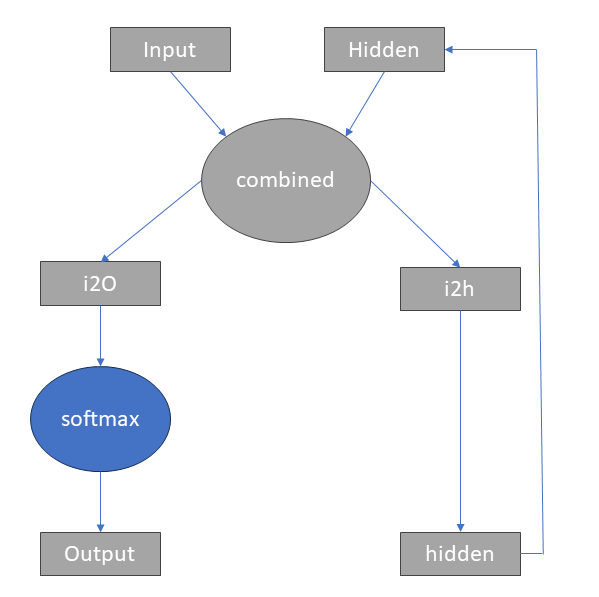
\includegraphics[width=0.50\linewidth]{nn_arch}
    %     \captionsetup{font=footnotesize}
    %     \captionof{figure}{Confusion Matrix}
    %     \label{fig:nn}
    % \end{Figure}
    

    \begin{enumerate}
        \item Input layer - \textit{n} number of unique words in collection of product names. Here, \textit{n} is the input layer size.  
        \item Hidden layers -  Transfers information from input node to the output node.
        \item Output layer - \textit{c} number of categories the model should predict.
        \item Softmax function - Takes input of \textit{K} real numbers, and normalizes it into a probability distribution consisting of \textit{K} probabilities.
    \end{enumerate}


    \vspace{0.5cm}
    \section{Evaluation and Results}
    \begin{enumerate}
        \item Preprocessing steps:-
        \begin{enumerate}
            \item Normalization of text: ngram vectorization to define vocabulary.
            \item To change \"A to A, apply the Normal form D (NFD).
            \item Use Beautiful Soup a Python library for pulling data out of HTLM and XML.
        \end{enumerate}

        
    \end{enumerate}

    \subsection{Text: Before and After normalization}
    \begin{center}
        \begin{tabular}{lll}
            \toprule 
                    &\textbf{Name} & \textbf{Category} \\ 
            \midrule
            \textbf{Before}&VAICO V10-4245 Stoßdämpfer & Stoßdämpfer \\
            \textbf{After}&vaico stoßdampfer & stoßdampfer \\
        
            \bottomrule
        \end{tabular}
        
    \end{center}
\columnbreak
    \subsection{Confusion Matrix}
    Confusion matrix displays how well the network performed on different categories. It is a matrix of actual categories (rows) which category the network guesses (columns).

    \begin{Figure}
        \centering
        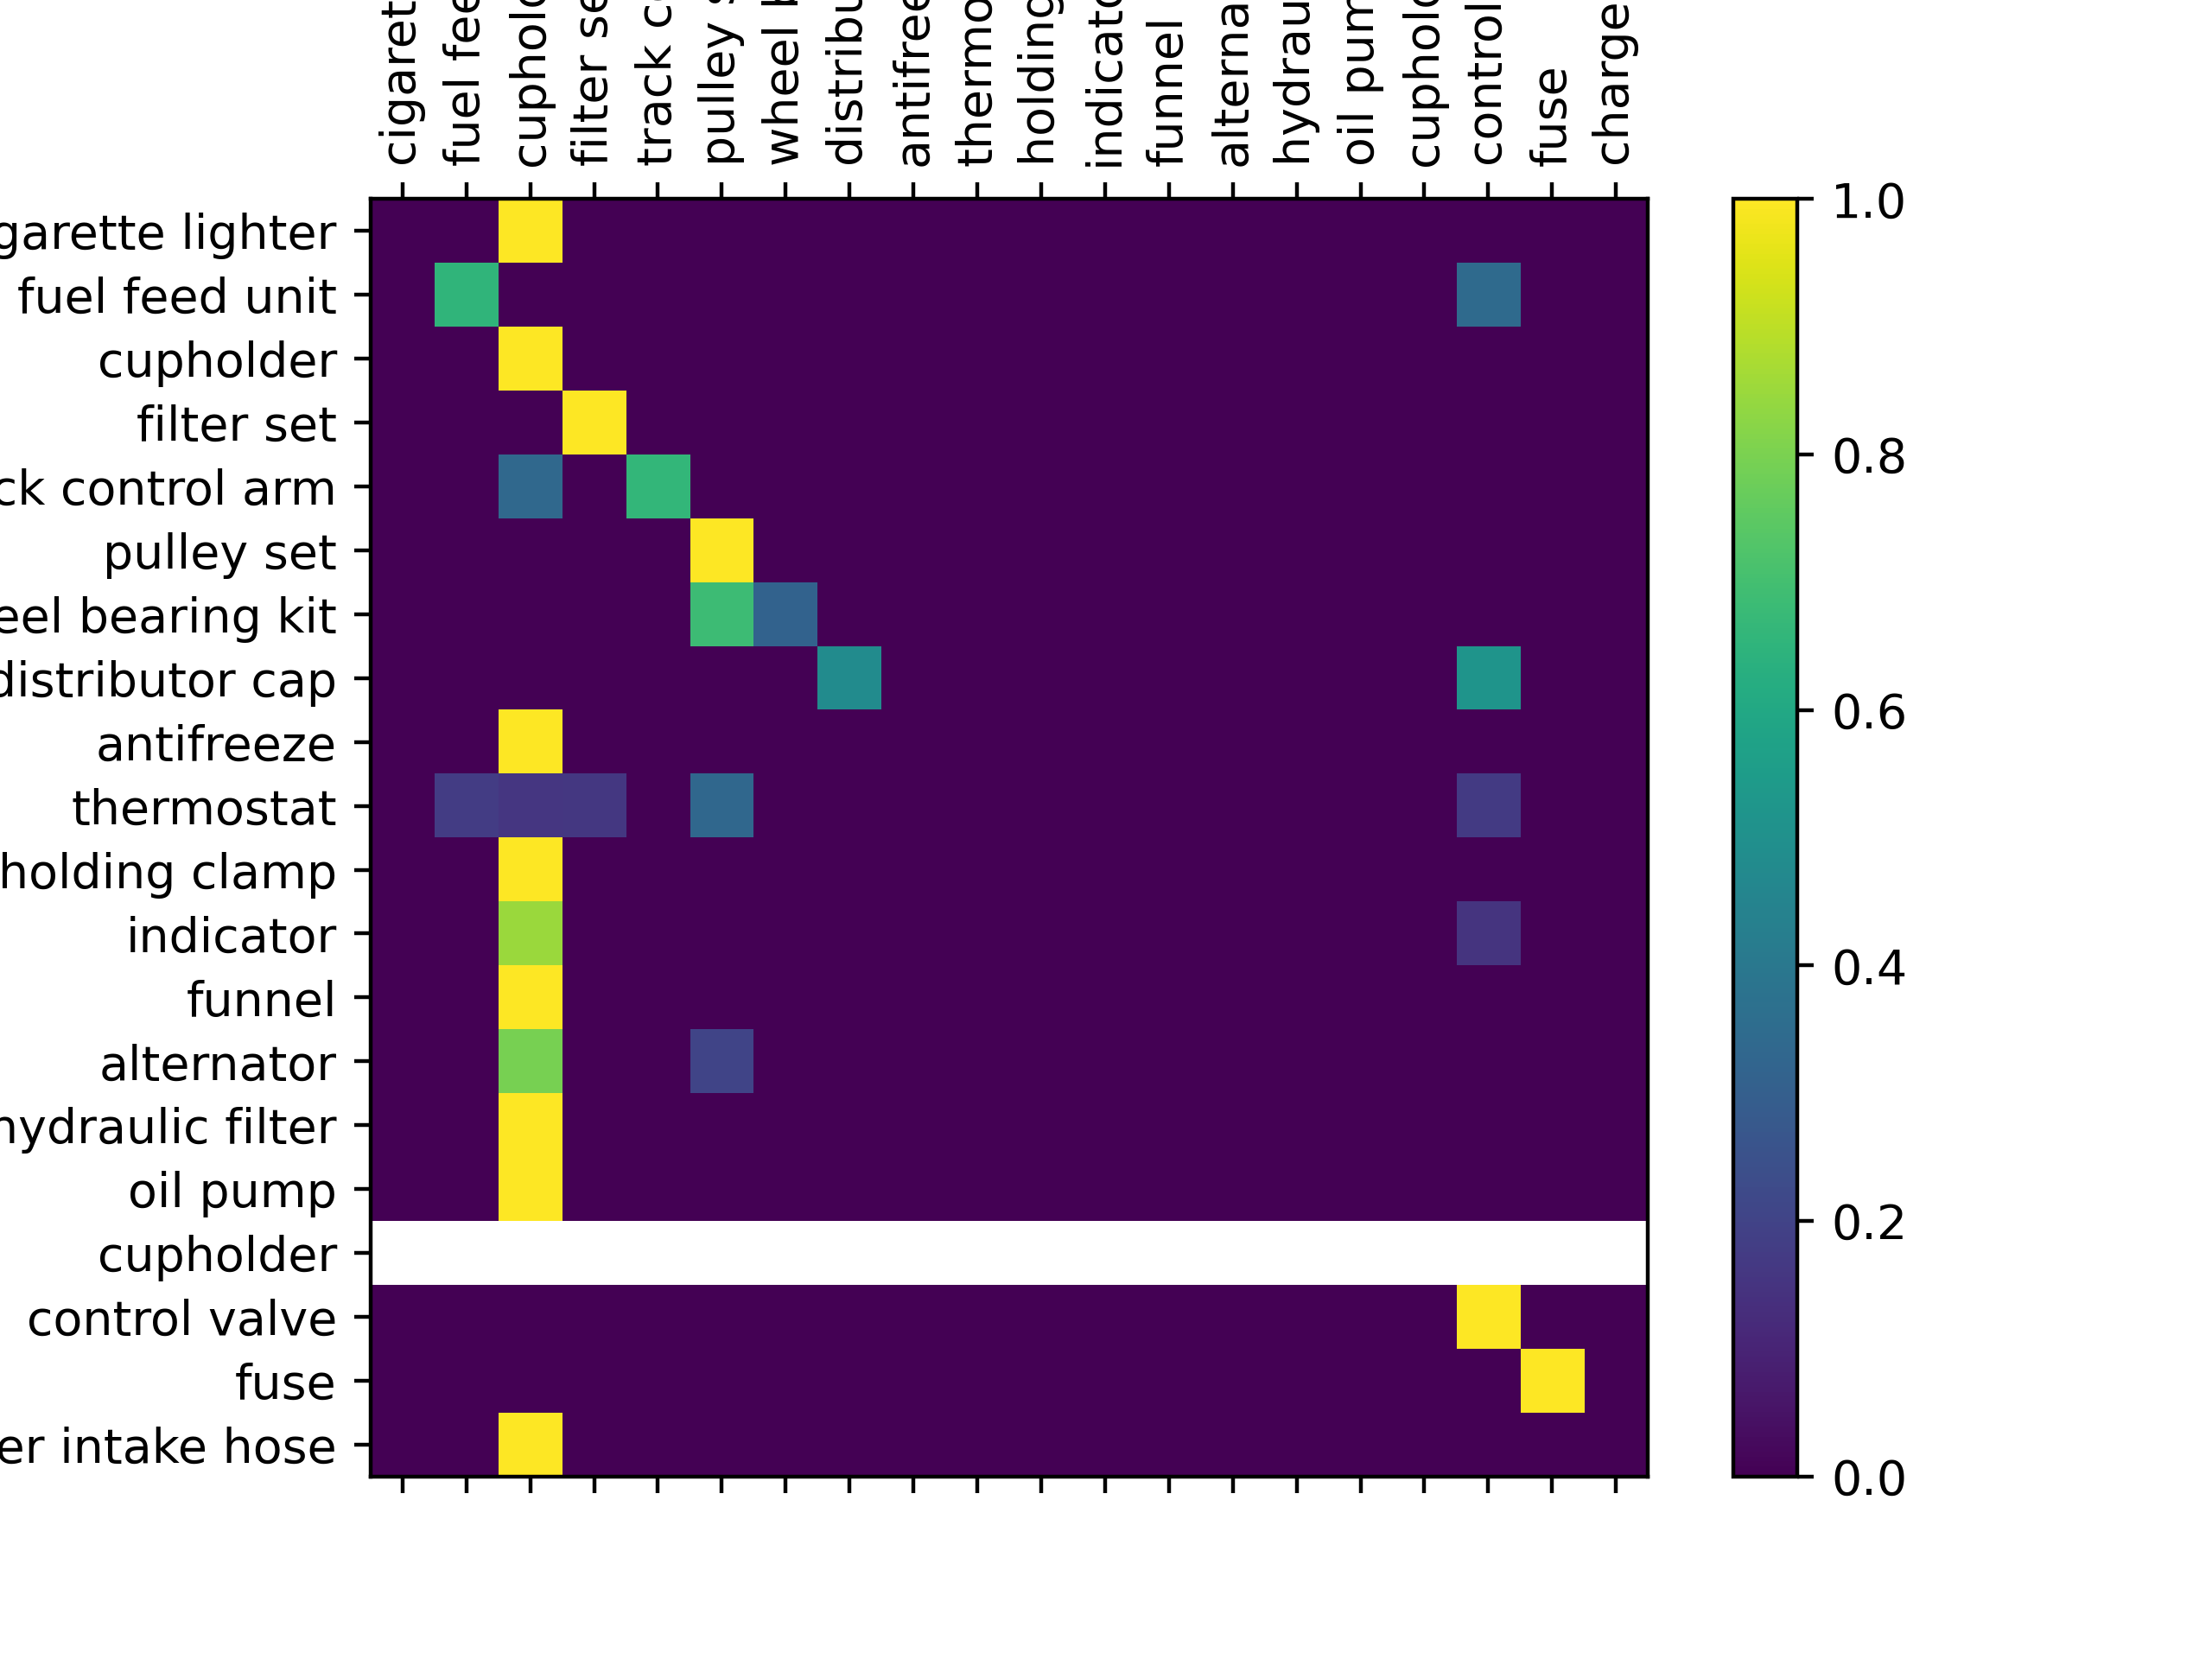
\includegraphics[width=0.50\linewidth]{confusion._200epoch}
        \captionsetup{font=footnotesize}
      
        \label{fig:cm}
    \end{Figure}


    \subsection{Negative log likelihood graph}
    The curve reaching 0 by end of training the machine learning model to 2,000,000 iteration indicates the model performed well.

    \begin{Figure}
        \centering
        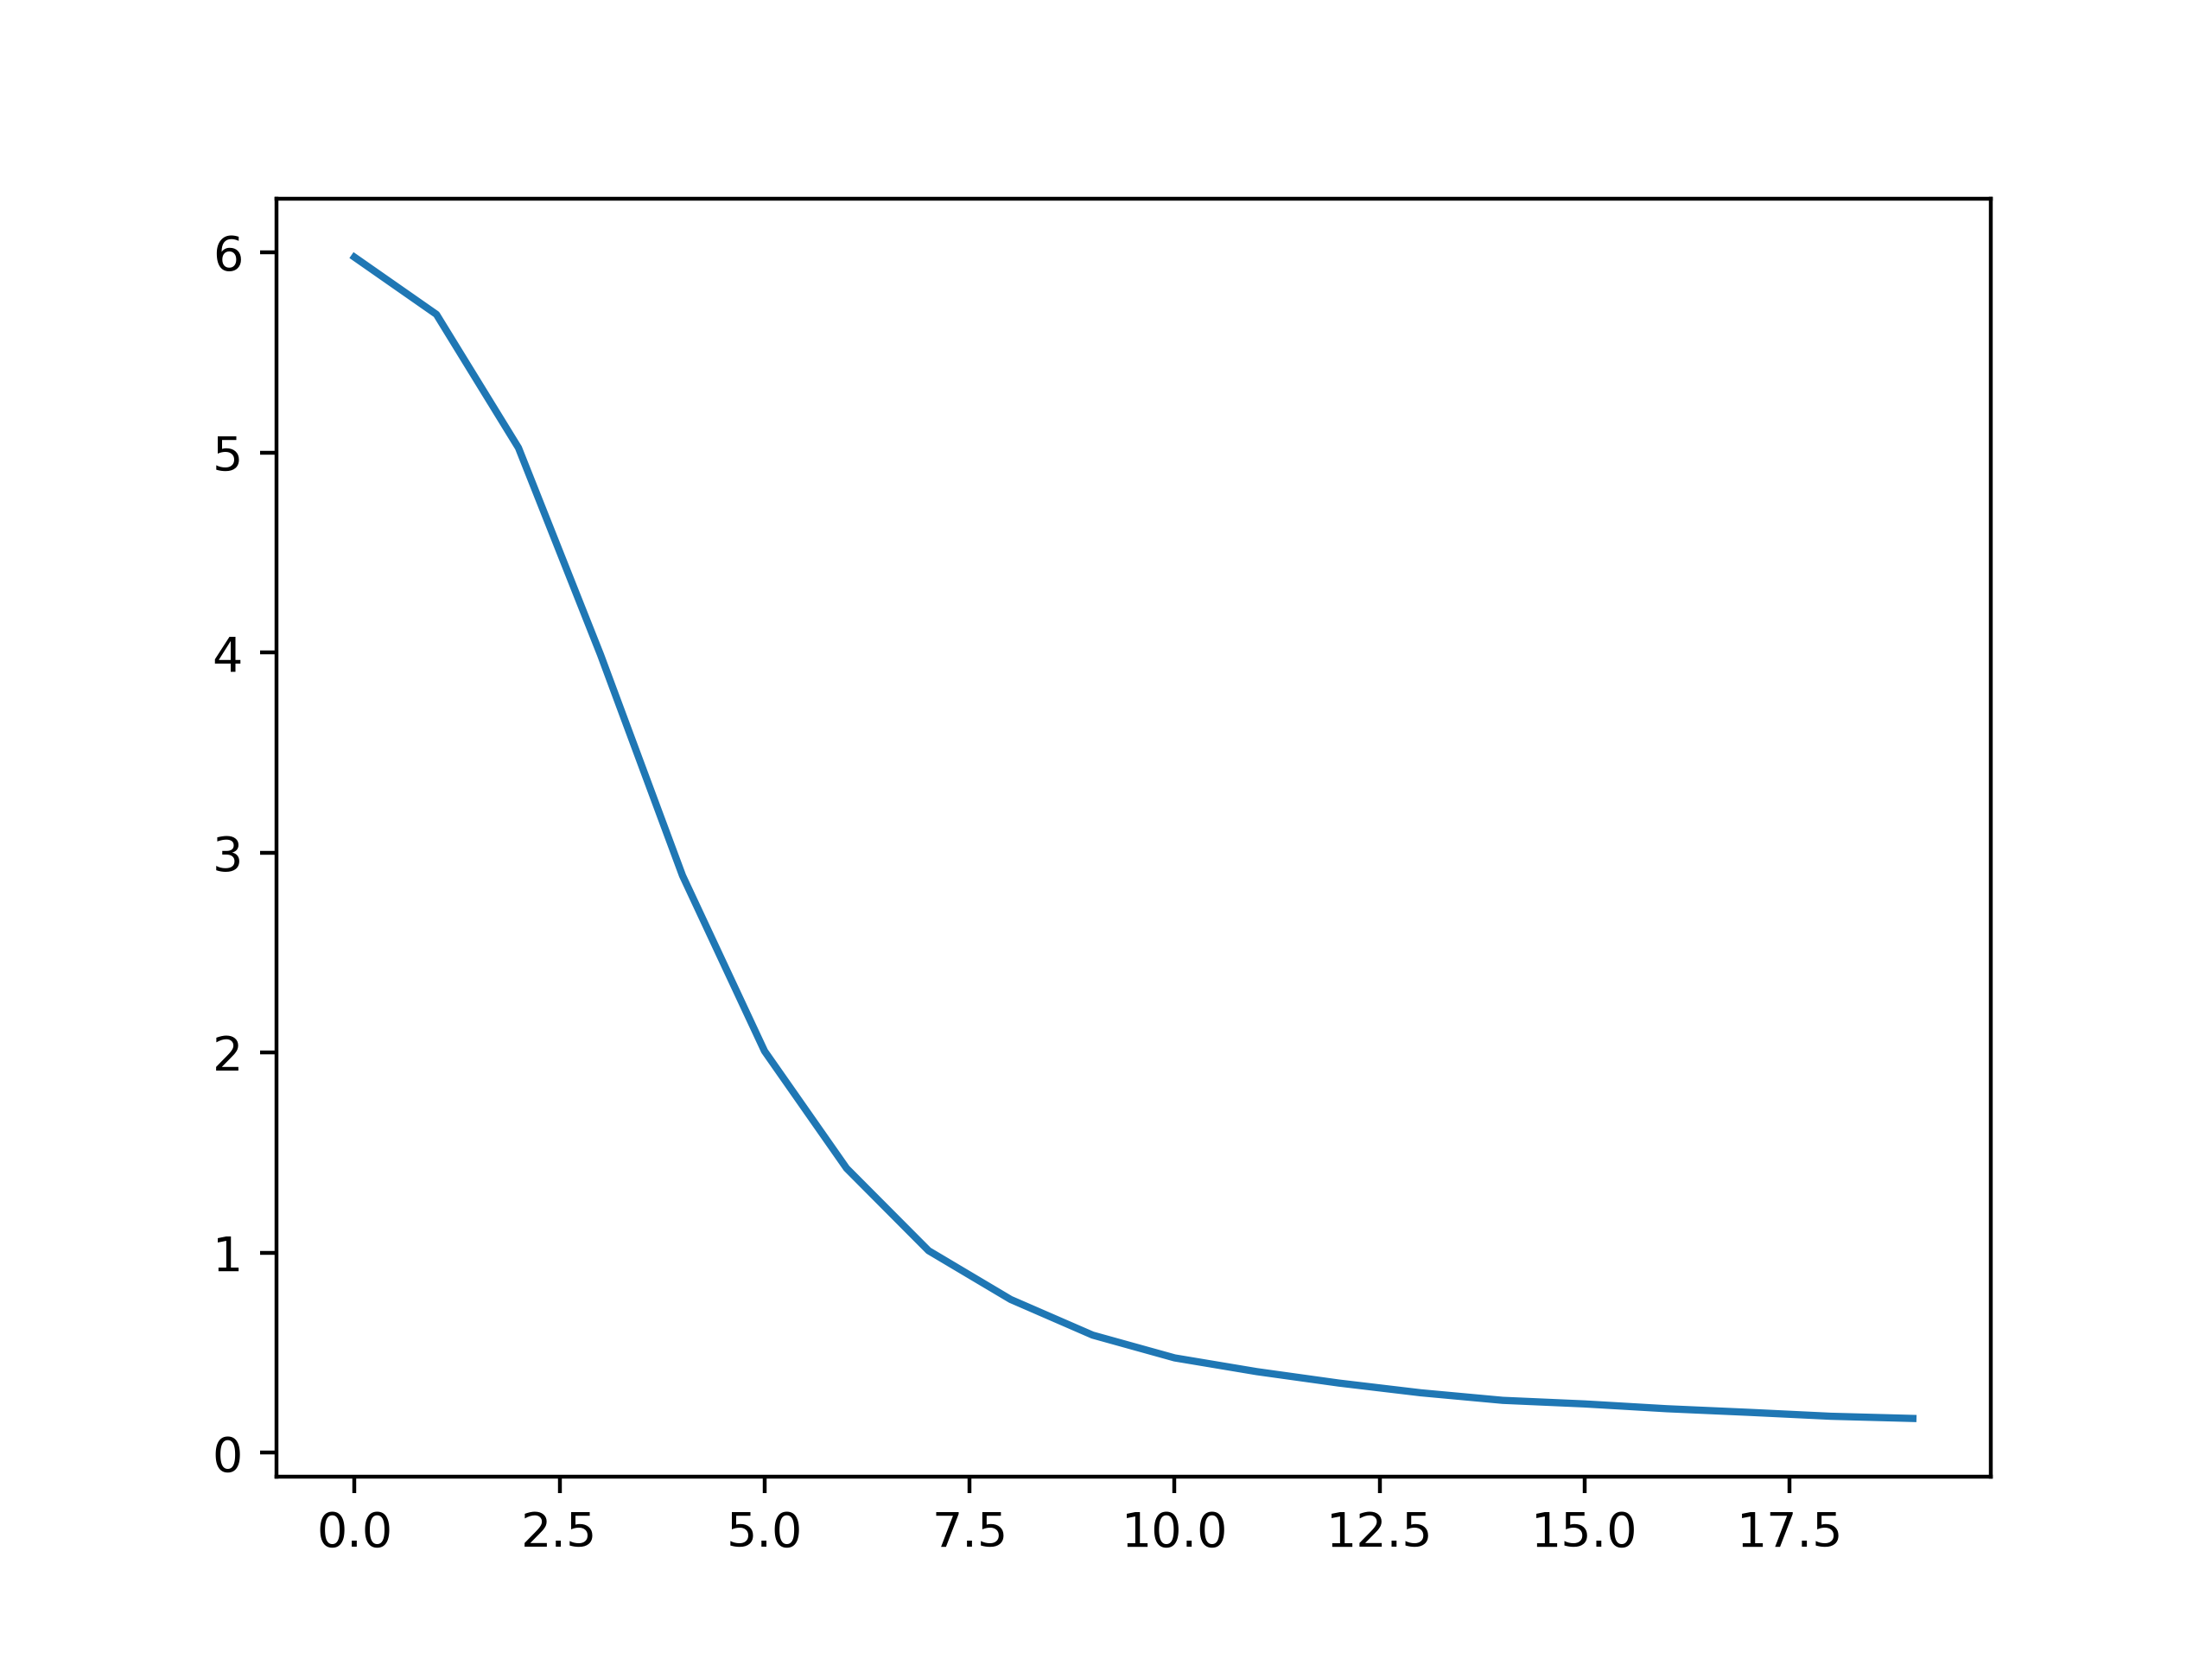
\includegraphics[width=0.50\linewidth]{loss}
        \captionsetup{font=footnotesize}
        
        \label{fig:loss}
    \end{Figure}

    \subsection{Actual vs predicted }
    Author tested the model with 10000 pairs of product name and category.
    Analyzing the falsely predicted result of 1455 records gained insight of incorrect categorization of existing products.
\vspace{0.5cm}

    \begin{center}
   \begin{tabular}{lll}
        \toprule 
            \textbf{Name} & \textbf{Category} & \textbf{Prediction} \\
        \midrule
            
            RPM Sensor, engine management&Sensor&rpm sensor \\
        
\bottomrule
   \end{tabular}
    \end{center}
        
\vspace{0.5cm}
%  \printbibliography

\section{References}

Buitinck, Lars et al. (2013).\\
\textit{API design for machine learning software: experiences from the scikit-learn project.}\\
\linebreak
Paszke, Adam et al. (2019).\\
\textit{PyTorch: An Imperative Style, High-Performance Deep Learning Library.}\\
\linebreak
Robertson, Sean (2023).\\
\textit{Classifying names with a character level RNN.}\\
\url{https://pytorch.org/tutorials/intermediate/char_rnn_classification_tutorial.html} 

    
\end{multicols*}
\end{document}